\documentclass[a4paper,12pt]{report}
\usepackage[utf8]{inputenc}
\usepackage[francais]{babel}
\usepackage{graphicx}
\usepackage{fancyhdr}
\usepackage[absolute]{textpos}
\usepackage[svgnames]{xcolor}
\usepackage{colortbl}
\usepackage{lastpage}
\usepackage{url}
\usepackage[hidelinks]{hyperref}
\usepackage{geometry}
\usepackage{tikz}
\usepackage{titlesec}
\usepackage{datetime}
\usepackage{lipsum}
\usepackage{supertabular}
\usepackage{float}
\usepackage[export]{adjustbox}
\usepackage{subcaption}
\usepackage{enumerate}
\usetikzlibrary{matrix}

\newcommand{\doctitle}{TD2}
\newcommand{\doclongtitle}{Technical documentation 2}

\title{\doctitle{} Vigilate}
\author{Soules Kévin, Mercier Daniel, Budowski Prune, Harscoat Morgane, Poncet Manuel, Keller Flavien}
\date{\today}


\definecolor{myBlue}{RGB}{23,54,93}
\definecolor{lightGray}{gray}{0.7}
\newdateformat{slashdate}{\twodigit{\THEDAY}/\twodigit{\THEMONTH}/\THEYEAR}
\newcolumntype{R}[1]{>{\centering\let\newline\\\arraybackslash\hspace{0pt}}m{#1}}

\titleformat{\section}[block]{\bfseries}{\thesection.}{1em}{}
\titleformat{\subsection}[block]{\hspace{2em}}{\thesubsection}{1em}{}
\titleformat{\subsubsection}[block]{\hspace{3em}}{\thesubsubsection}{1em}{}
  
\geometry{
  a4paper,
  left=20mm,
  right=20mm,
}

\setlength{\unitlength}{1mm}
\addtolength{\headheight}{1.5\baselineskip}
\renewcommand{\headrulewidth}{0.0pt}
\renewcommand{\footrulewidth}{0.4pt}


\fancypagestyle{eip}{
  \fancyhf{}
  \fancyhead[L] {
    \includegraphics[width=3cm]{../../../logos/logo_eip.png}
  }
  \fancyhead[R] {
    \colorbox{myBlue}{
      \textcolor{white}{
        \Large \textbf{[2017][Vigilate][\doctitle{}]}
      }
    }
  }
  \renewcommand{\headrulewidth}{0pt}
  \fancyfoot[L]{
    \textcolor{gray}{
      \{EPITECH.\}
    }
  }
  \fancyfoot[C]{Vigilate}
  \fancyfoot[R]{
    \ifnum\value{page}>0
    \thepage/\pageref{LastPage}
    \fi
  }
}

\makeatletter
\let\ps@plain\ps@eip
\makeatother

\pagestyle{eip}


\begin{document}
\date{\slashdate\today}
\setcounter{page}{-3}

% --- (1) Page de garde ---

\thispagestyle{empty}
\vspace*{\stretch{2}}
\begin{center}
  \textcolor{myBlue}{\Huge \textbf{EIP Vigilate}}\linebreak
  \vspace*{\stretch{1}}
  \textcolor{gray}{\textit{\Large \doclongtitle{} (\doctitle{})}}\linebreak
  \vspace*{\stretch{1}}
  {\today}
\end{center}
\vspace*{\stretch{1}}
\newpage

% --- (2) Résumé ---

\vspace*{\stretch{1}}
\begin{flushleft}
  \textcolor{myBlue}{\textit{\large \textbf{Résumé du document}}}\linebreak
\end{flushleft}
Le cahier des charges commence par un bref rappel de notre EIP, Vigilate, un outil de sécurité informatique qui permet de se tenir informé des dernières vulnérabilités publiques rapidement sur tous les programmes que l’utilisateur souhaite vérifier. On mettra en avant les contraintes fonctionnelles et les exigences non-fonctionnelles comme le fait que notre projet doit être sécurisé, ou alors la réactivité de notre outil. Notre projet est réalisé par 6 personnes. Le document présente d’une part la structure du projet : un site web, le back-end, une machine virtuelle et un scanneur de programme et d’autre part, les différentes fonctionnalités du projet à partir d’un document UML (connexion de l’utilisateur, possibilité de modifier ses préférences : programmes à surveiller, style d’alerte souhaité...). Nous présentons dans la partie 6 l’organisation prévue : 2 personnes sur le site web, 2 sur le back-end, 1 sur la machine virtuelle et 1 sur le scanneur de programme. Ainsi que la méthodologie utilisée, basée sur la méthode Agile (Scrum). Pour ce faire, nous devons construire un produit backlog avant de commencer à développer le projet, puis organiser un nombre de sprints adéquat, d’une durée relativement courte (principe de la méthode agile) mais qui permettront d’avoir un projet fonctionnel à chaque fin de sprint avec chaque tâche décrite dans un backlog de sprint. Nous présenterons également l’environnement et les outils utilisés (github pour héberger nos documents...). Nous avons réalisé un template de mise en page pour toute notre documentation avec Latex. Nous avons choisi de respecter la norme Python Pep8 pour le développement. Dans une dernière partie, nous proposerons une description des tests, utilisés pendant le développement notamment grâce à l’outil Travis et les tests une fois l’outil terminé.\\
\vspace*{\stretch{1}}
\newpage

% --- (3) Cartouche + révisions ---

\begin{flushleft}
  \vspace*{\stretch{1}}
  \textcolor{myBlue}{\textit{\large \textbf{Description du document}}} 
  \bigbreak
  \begin{tabular}{|>{\columncolor[RGB]{220,220,220}\color{Navy}\bfseries}l|p{12cm}|}
\hline
Titre & [2017][Vigilate][\doctitle{}] \\
\hline
Date & 31/01/2015 \\
\hline
Auteur & Kévin SOULES \\
\hline
Responsable & Kévin SOULES\\
\hline
Email & vigilate\_2017@labeip.epitech.eu\\
\hline
Sujet & \doclongtitle{}\\
\hline
Mots clés & \doctitle{}, sécurité, vulnérabilités\\
\hline
Version du modèle & 1.1\\
\hline
\end{tabular}


  \vspace*{\stretch{2}}
  \bigbreak
  \bigbreak
  \textcolor{myBlue}{\textit{\large \textbf{Tableau des révisions}}}
  \bigbreak
  \small
\begin{tabular}{|p{1.5cm}|l|p{2.5cm}|p{7.8cm}|l|}
  \hline
 
   \rowcolor{Gainsboro}Date  & Auteur & Section(s) & Commentaires \\
  \hline
24/01/15 & Kévin Soules &  & Création du documents\\
  \hline
27/01/15 & Kévin Soules & Chapitre 1 et 2.1 & Recherche de liste de solutions. Rédaction du texte d'un premier concurrent. Remplissage des rappels.\\
\hline
28/01/15 & Prune Budowski & Chapitre 1 & Amélioration des rappels \\
\hline
29/01/15 & Prune Budowski & Chapitre 3.3.2 & Rédaction de la partie ``Ce qui ne sera pas couvert''\\
\hline
29/01/15 & Daniel Mercier & Chapitre 2.2 & Rédaction du texte du deuxième concurrent.\\
\hline
29/01/15 & Kévin Soules & Chapitre 2.3 & Rédaction du texte du troisième concurrent. \\
\hline
30/01/15 & Morgane Harscoat & Chapitre 2.4 & Début de rédaction du texte du quatrième concurrent. \\
\hline
30/01/15 & Kévin Soules & Chapitre 2.5 & Rédaction du texte du cinquième concurrent.\\
\hline
31/01/15 & Kévin Soules & Conclusion, Glossaire & Matrice de préférence.Rédaction d'un glossaire. \\
\hline
31/01/15 & Prune Budowski & Résumé, Conclusion, Chapitre 3.1 & Rédaction du résumé. SWOT. Rédaction de la partie ``Ce que vous apportez''.  
  \\
\hline
31/01/15 & Daniel Mercier & Toutes & Corrections. \\
31/01/15 & Prune Budowski & & Mise en page. \\
31/01/15 & Kévin Soules & & Mise en page.
\\
  \hline
\end{tabular}
\normalsize

  \vspace*{\stretch{1}}
\end{flushleft}

% --- (4) Tables des matières ---

\tableofcontents




\textcolor{myBlue}{\chapter{Introduction}}
\section{Vue du projet}
Notre projet est découpé en plusieurs blocs: (cf Figure 1.1)\\
\begin{itemize}
\item Le programme de scan est un programe qui peut être installé sur la machine pour automatiser l'envoi des données sur notre service
\item Le backend est le coeur de la solution
\item Le site web correspond à la partie visible par l’utilisateur
\item La machine virtuelle est une installation indépendante de notre solution permettant à un utilisateur n’avoir une copie de notre solution dont il a le contrôle.
\end{itemize}

\begin{figure}[H]
  \centering
  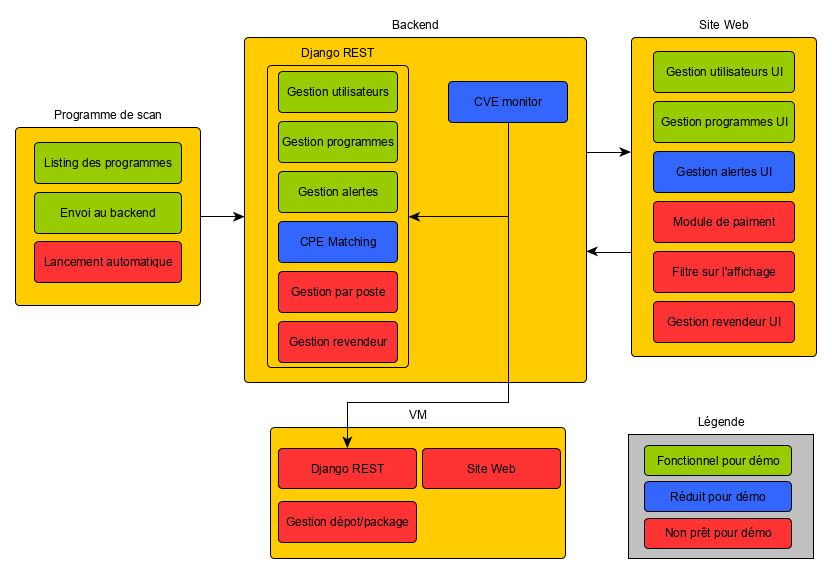
\includegraphics[width=14cm]{block_diagram.png}
  \vspace*{0.5cm}
  \caption{Vue projet}
  \vspace*{1cm}
\end{figure}

\section{Vue logique}
Sur ce schéma (Figutr 1.2), on peut voir l’interaction entre les classes principales.\\
\begin{itemize}
\item La classe Alert contient la liste des aletes actives.
\item La classe UserPrograms contient la liste des programmes sur lesquels un utilisateur veut recevoir des alertes.
\item La classe User contient les informations personnelles d’un utilisateur.
\item La classe Reference contient la liste des références utilisé par les vulnérabilitées.
\item La classe Cve contient la liste de vulnérabilité connue de notre service.
\item La classe Cpe contient la liste de programmes/version connue par notre service.
\item La classe Cwe contient la liste des descriptions de vulnérabilitée.

\end{itemize}

\begin{figure}[H]
  \centering
  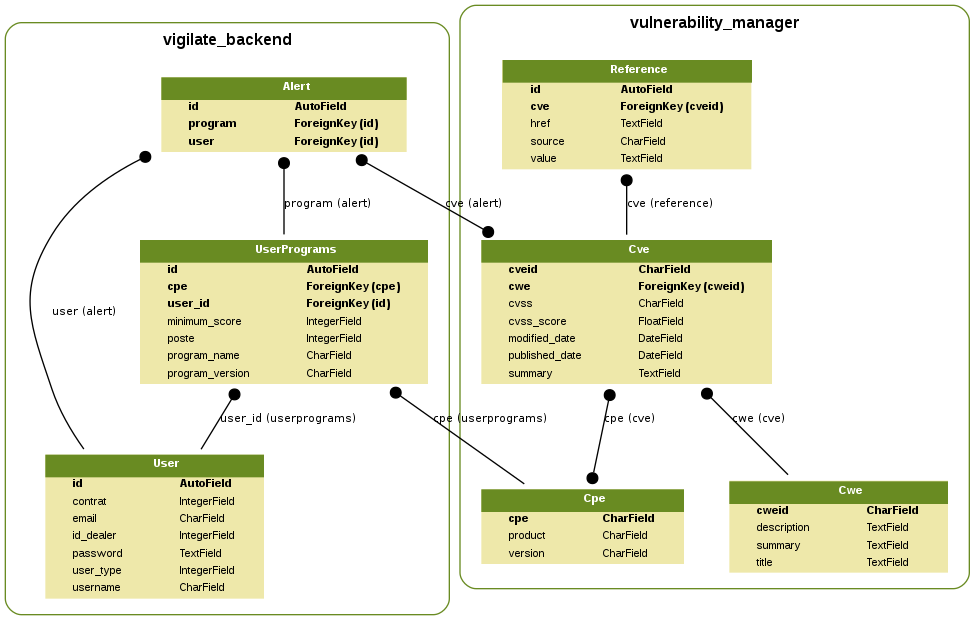
\includegraphics[width=16cm]{django_class.png}
  \vspace*{0.5cm}
  \caption{Vue Logique}
  \vspace*{1cm}
\end{figure}


\section{Norme du code}
Le langage de programmation utilisé au sein de notre solution est majoritairement python. Nous avons donc choisi de respecter la norme pep8 étant la norme recommandé pour ce langage.

\section{Tests et conditions de passage du dev à une release}
Chaque commit reçu sur le github du projet lance une suite de test d’intégration continue via travis.
Avant d’être accepté comme release, une version de dev passera par une validation via un audit de sécurité. Cet audit contiendra entre autres des test via de l’analyse static de code, des tests de scanneur web, et du fuzzing.
À partir du moment où il est décidé de fournir une release, les nouvelles features ne seront plus accepté (“freeze” de la version). En contrepartie, les issues connus et listé sur le bugtracker seront résolu afin d'augmenter la qualité du produit.
\section{Stratégie de release}
Quand une release sera prête, un tag github sera crée pour marquer cet état d’avancement.
Un exécutable windows sera crée pour le scanner de programme. (script python avec interpréteur python embarqué)
vue du projet via un schéma de haut niveau
Notre projet est découpé en plusieurs blocs:
Le site web correspond à la partie visible par l’utilisateur
Le programme de scan est un programe qui peut être installé sur la machine pour automatiser l'envoi des données sur notre service
Le backend est le coeur de la solution
La machine virtuelle est une installation indépendante de notre solution permettant à un utilisateur n’avoir une copie de notre solution dont il a le contrôle.
\textcolor{myBlue}{\chapter{Développement}}
\section{Github}
Le projet est hébergé sur github. Nous utilisons plusieurs fonctionnalitées de cette outil:
\begin{itemize}
\item Gestion de versions (git)\\
Github nous permet simplement de développer à plusieurs sur un même code.
\item Issue
Nous utilisons les Issues pour lister les bugs et/ou features relatives à notre projet.
\item Milestone
Nous utilisons les Milestone pour préciser si une issue doit être incluse dans la prochaine deadline ou pas.
\item Pull Request
Nous utilisons les Pulls Request pour proposer des changement sur le code.
\end{itemize}

\section{Méthodologie}
Que ce soit pour résoudre une issue, pour ajouter une fonctionnalité, ou même pour changer quelques lignes de codes, une branche dédiée tout être utilisé. Par exemple, si une issue numéro \#42 signale qu'il y a un bug sur la connexion des utilisateurs, le développeur qui va se charger de réparer ce bug créera une branche avec un nom similaire à ``issue-42-connexion-utilisateur''.\\
\\
Une fois les commits push sur cette branche, le développeur peut voir si les tests d'intégrations travis sont passés. Si c'est le cas, le développeur crée alors une Pull Request pour proposer ses changements sur Master.\\
À ce moment-là, un des développeurs principaux vérifie les changements effectués, vérifie que les tests unitaires passent et que la couverture de test n'a pas baissé. Si tout est en règle, alors il peut accepter cette Pull Request. Dans le cas contraire, il indiquera à la personne ayant envoyé la Pull Request pourquoi elle n'a pas été acceptée.
\textcolor{myBlue}{\chapter{Documentation}}
\section{Documentation API}
La documentation de l'API est disponible à cette adresse: https://github.com/vigilate/backend/blob/master/api.md
\section{Documentation généré}
La documentation à générée est disponible à cette adresse: https://github.com/vigilate/backend/tree/master/docs






\end{document}